\centering{\textbf{ค่าความเร่งเนื่องจากแรงโน้มถ่วงนี้สามารถนำไปใช้คำนวณได้โดยถือหลักการดังนี้}}
\tcblower
\begin{minipage}{.6\textwidth}
\begin{itemize}[leftmargin=*]
	\item[1)] ขณะวัตถุกำลังเคลื่อนที่ขึ้น \hfill  ให้ใช้ค่าความเร่งเป็น \\–9.8  เมตร/วินาที$^2$  เพราะความเร่งนี้มีทิศลงตรงกันข้ามกับความเร็วของการเคลื่อนที่ซึ่งมีทิศขึ้น
	\item[2)] ขณะวัตถุกำลังเคลื่อนที่ลง \hfill  ให้ใช้ค่าความเร่งเป็น \\+9.8  เมตร/วินาที$^2$       เพราะความเร่งนี้มีทิศลงเหมือนกับความเร็วของการเคลื่อนที่
	\item[3)] หากวัตถุเคลื่อนที่ขึ้นในแนวดิ่ง  ขณะวัตถุอยู่ที่จุดสูงสุดของการเคลื่อนที่จะมีความเร็วในแนวดิ่งเป็นศูนย์เสมอ 
\end{itemize}
\end{minipage}
\hfill
\begin{adjustbox}{valign=c} \begin{minipage}[t]{.35\linewidth}
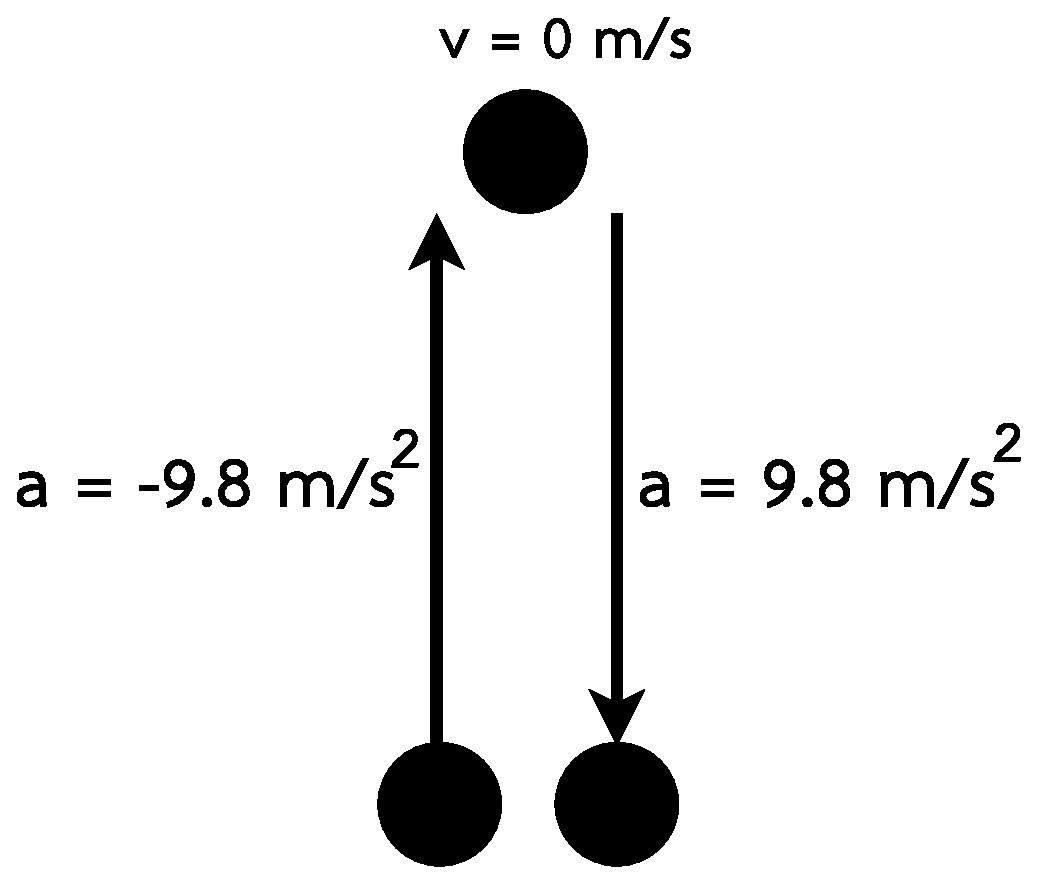
\includegraphics[width=\linewidth]{content-7.eps}
\end{minipage}
\end{adjustbox}
